\section{Применение ``CATIA-GDML geometry builder'' за пределами CBM RICH}\label{sec:secBuilderOtherUsage}

\subsection{CBM ECAL frame}

%\centering

\begin{figure}[H]
\begin{minipage}[b]{0.31\textwidth}
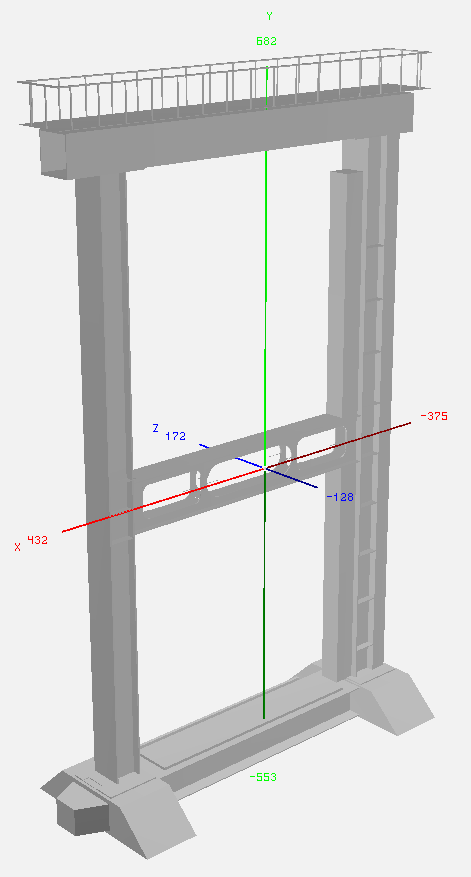
\includegraphics[width=0.95\textwidth]{pictures/ECAL_SIS300_ROOT.png}
\caption{}
\label{fig:CbmEcal1}
\end{minipage}
\hspace{0.01\textwidth}
\begin{minipage}[b]{0.31\textwidth}
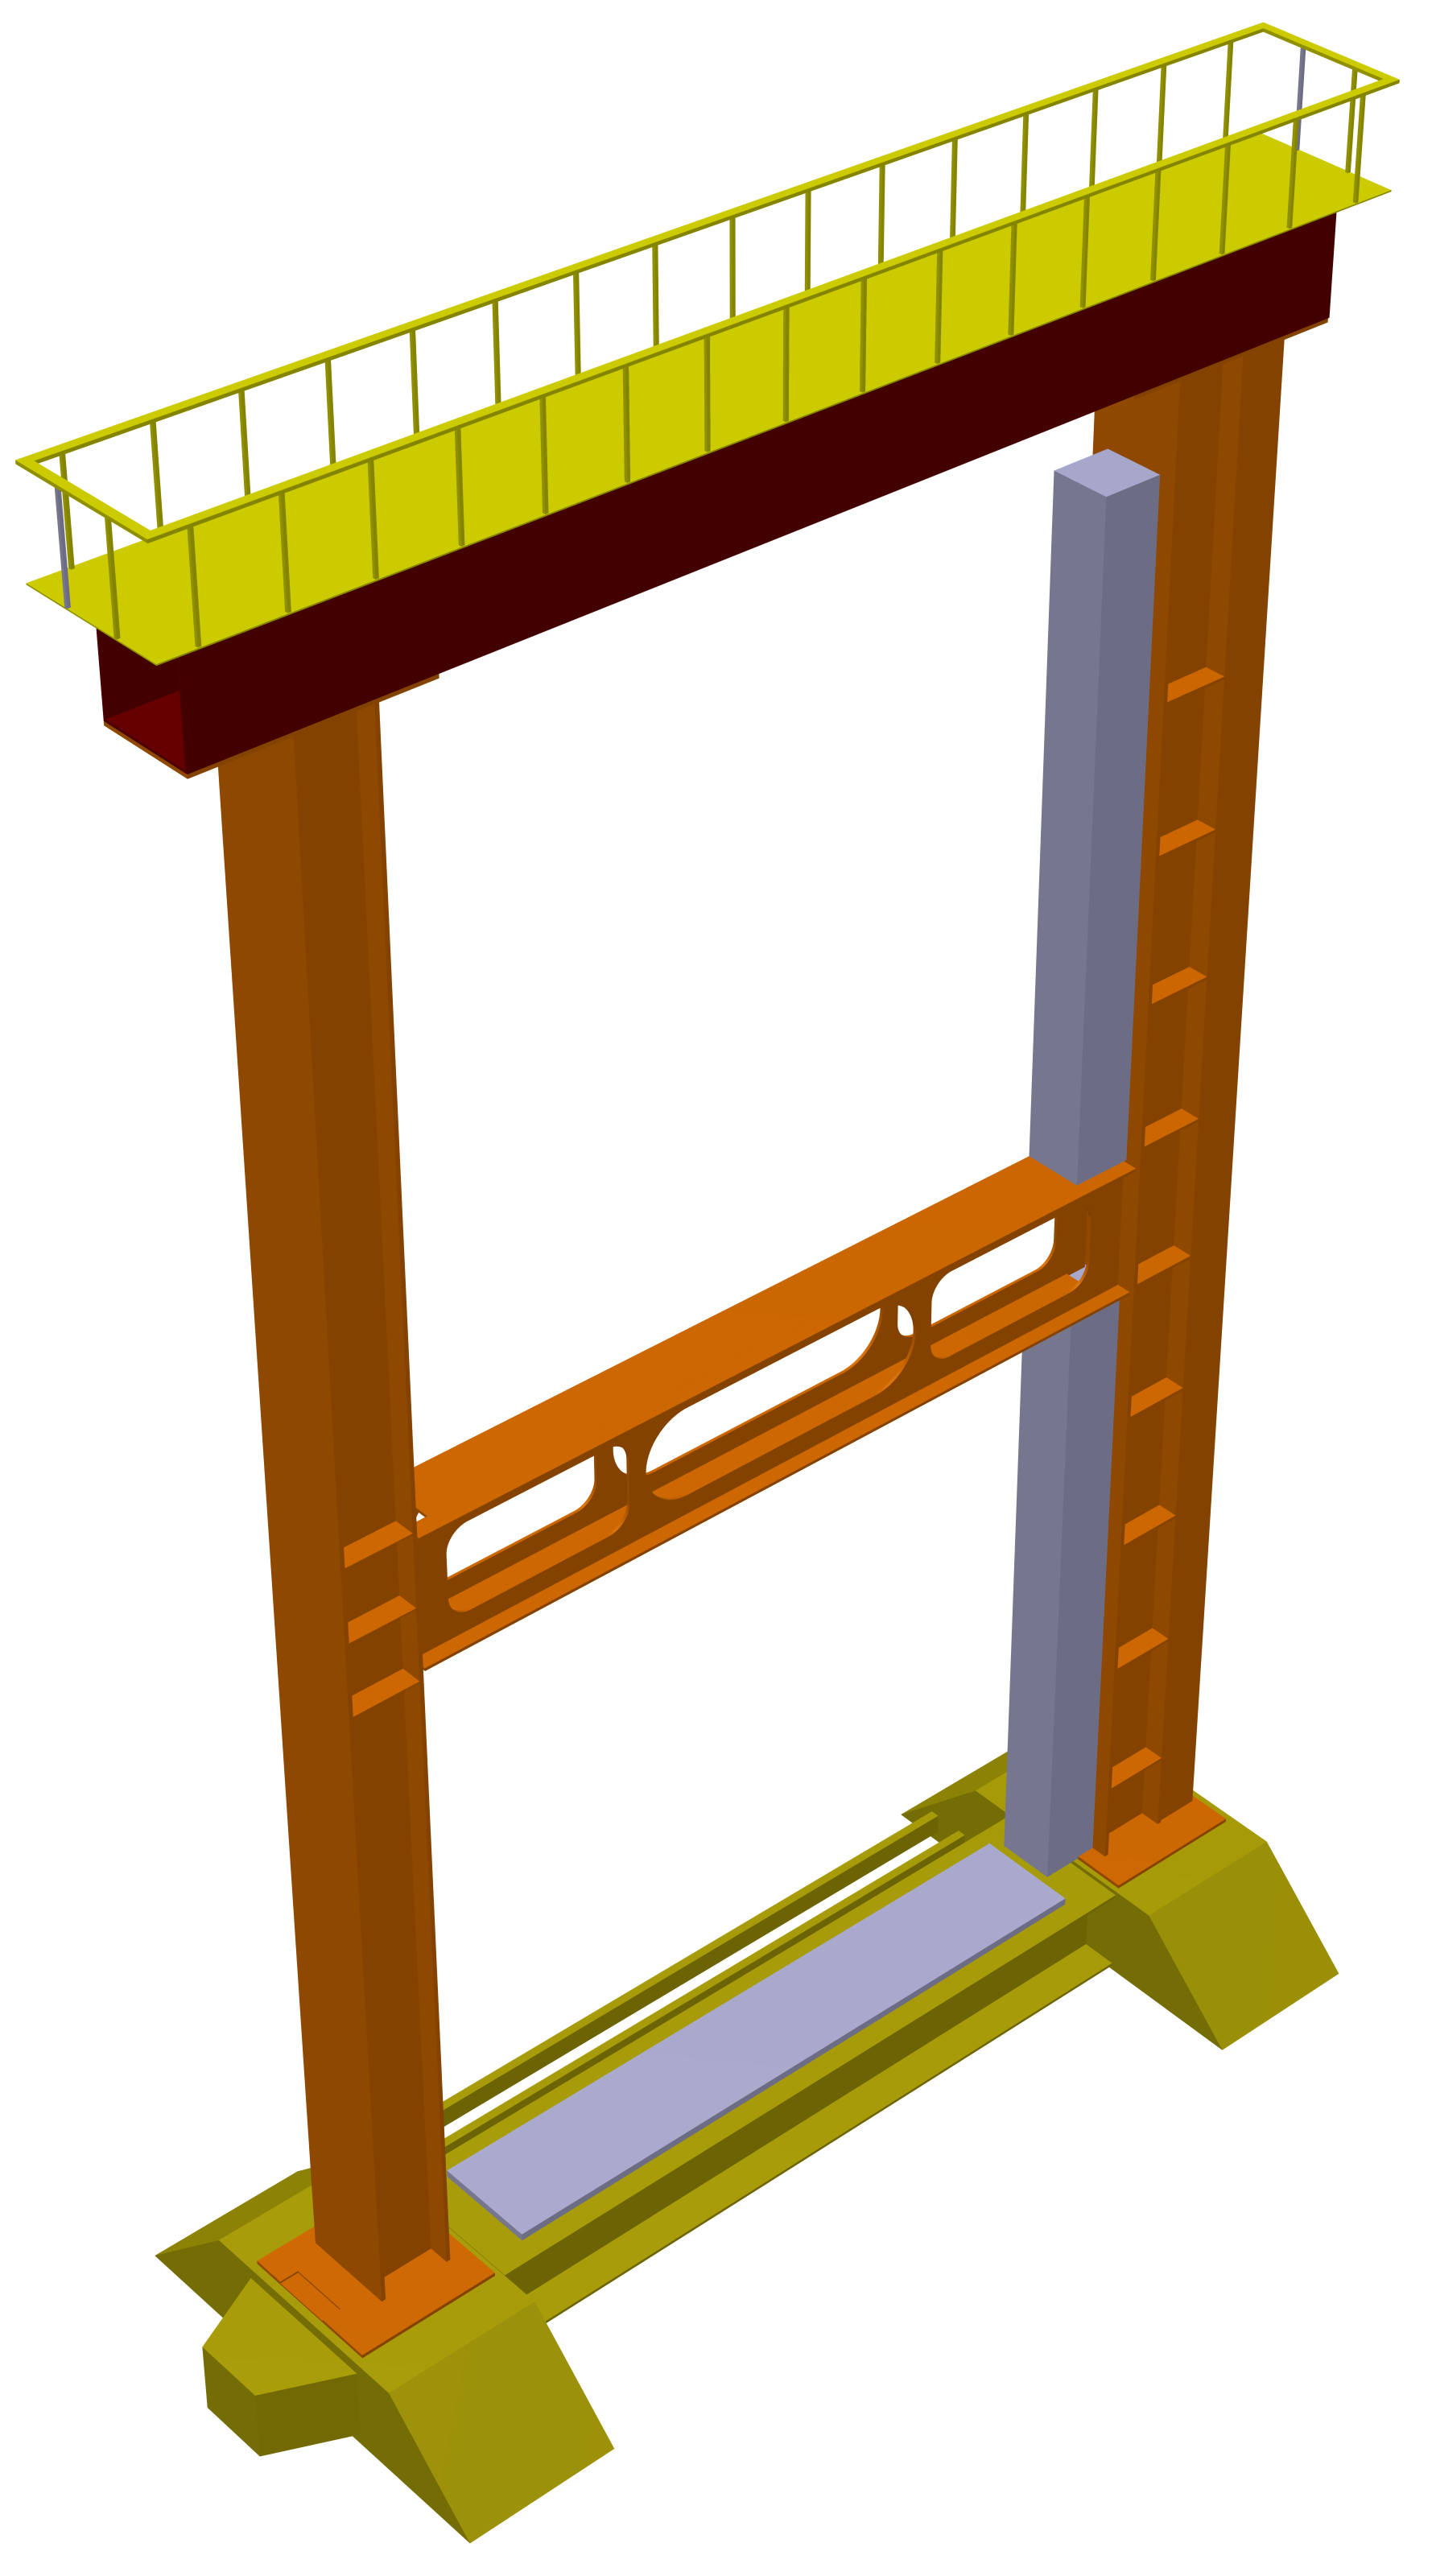
\includegraphics[width=0.95\textwidth]{pictures/ECAL_SIS300_CATIA_g4.png}
\caption{}
\label{fig:CbmEcal2}
\end{minipage}
\hspace{0.01\textwidth}
\begin{minipage}[b]{0.31\textwidth}
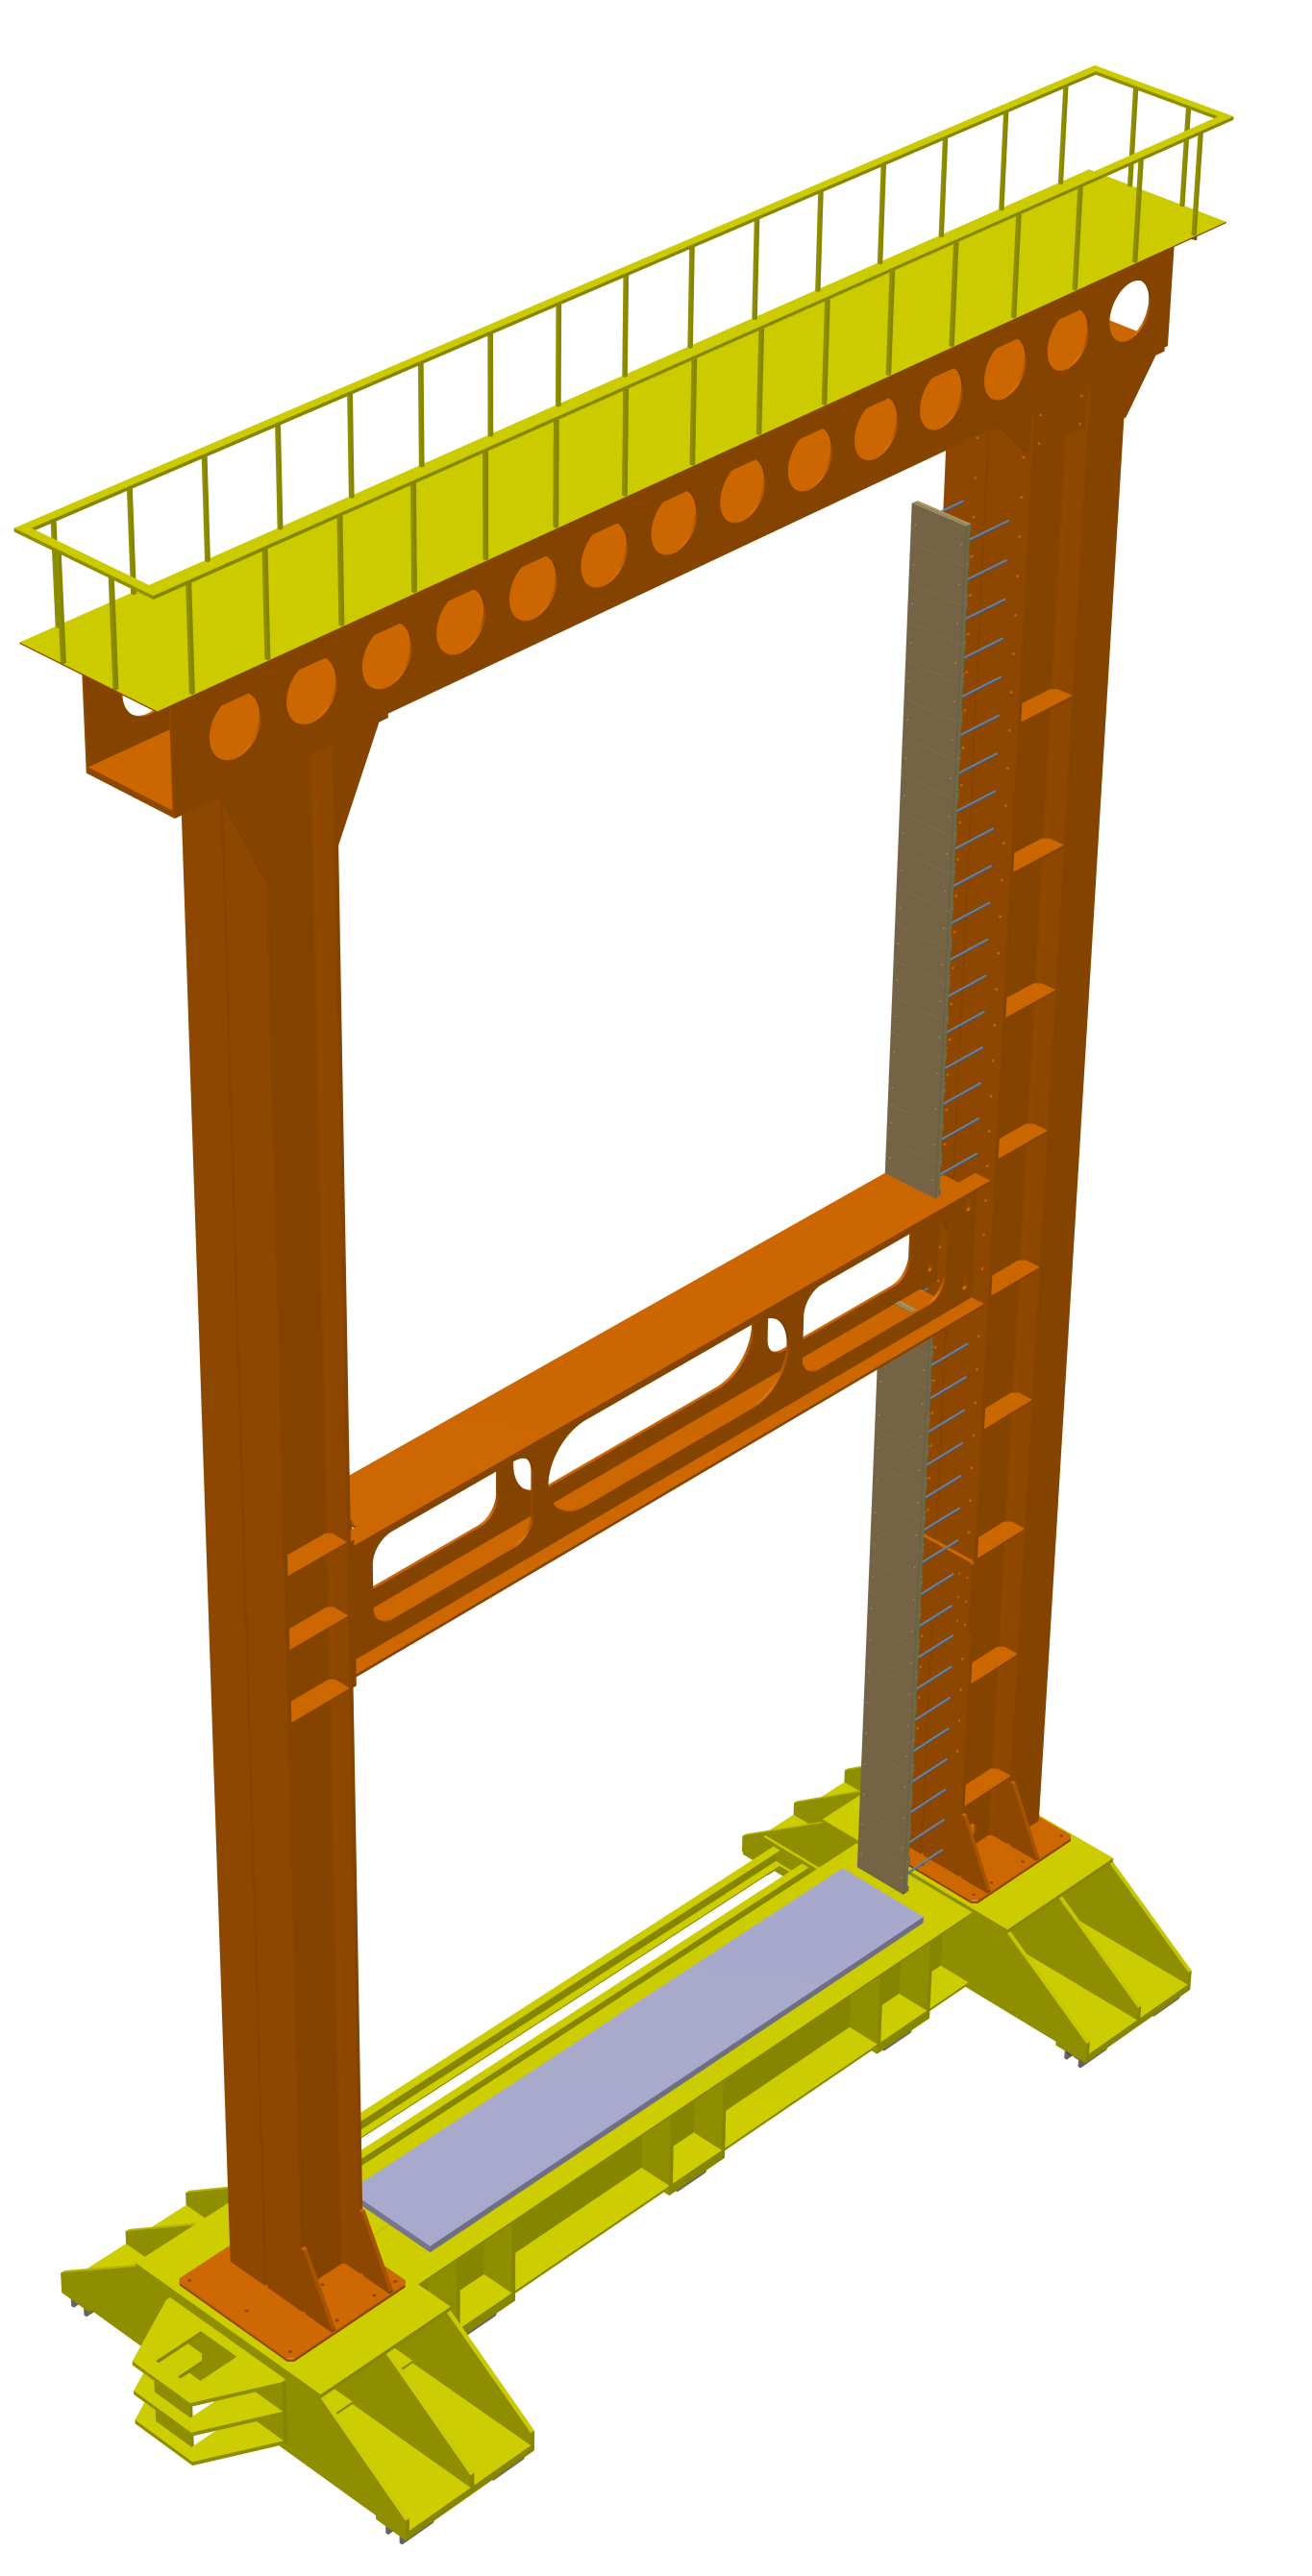
\includegraphics[width=0.95\textwidth]{pictures/ECAL_SIS300_CATIA_cad.png}
\caption{}
\label{fig:CbmEcal3}
\end{minipage}
\end{figure}

\subsection{Магнит CBM}

\begin{figure}[H]
\begin{minipage}[b]{0.495\textwidth}
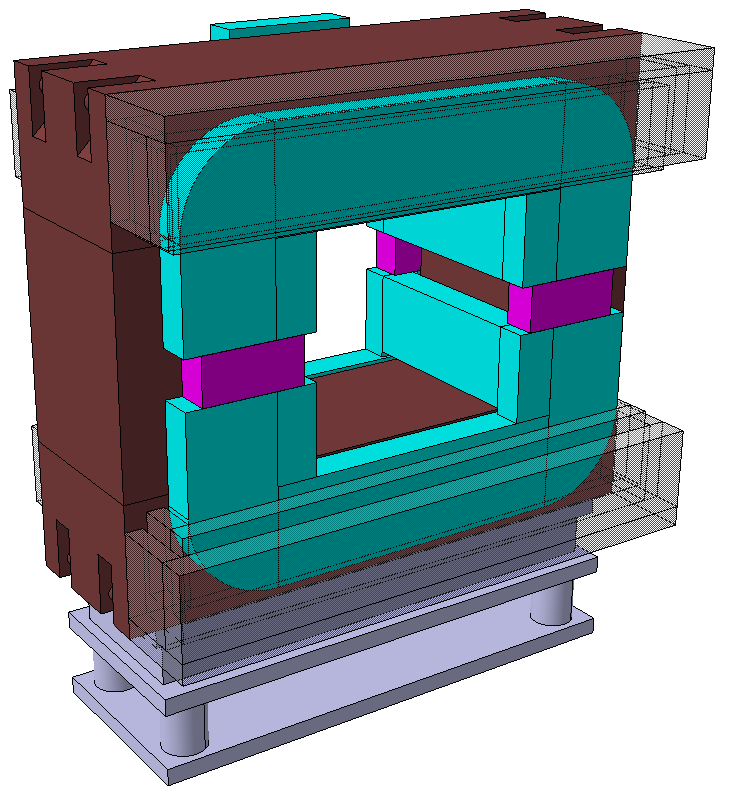
\includegraphics[width=0.95\textwidth]{pictures/Old_magnet_2.png}
\caption{}
\label{fig:OldCbmMagnet1}
\end{minipage}
\hspace{0.01\textwidth}
\begin{minipage}[b]{0.495\textwidth}
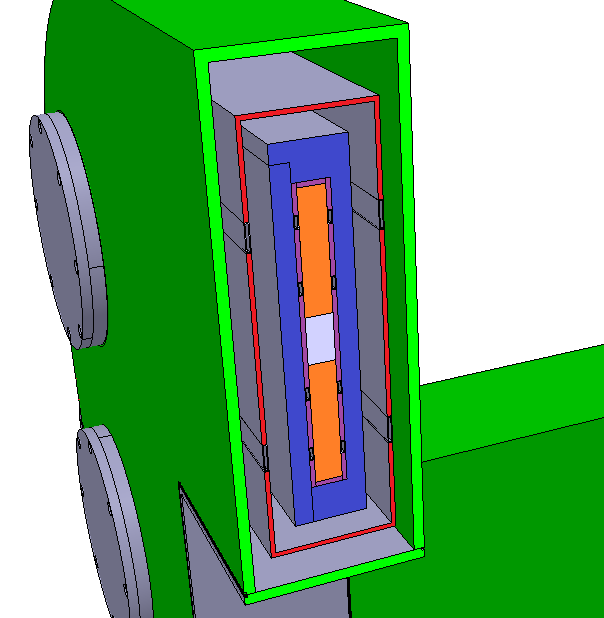
\includegraphics[width=0.95\textwidth]{pictures/Old_magnet_coils.png}
\caption{}
\label{fig:OldCbmMagnet2}
\end{minipage}
\end{figure}

\begin{figure}[H]
\centering
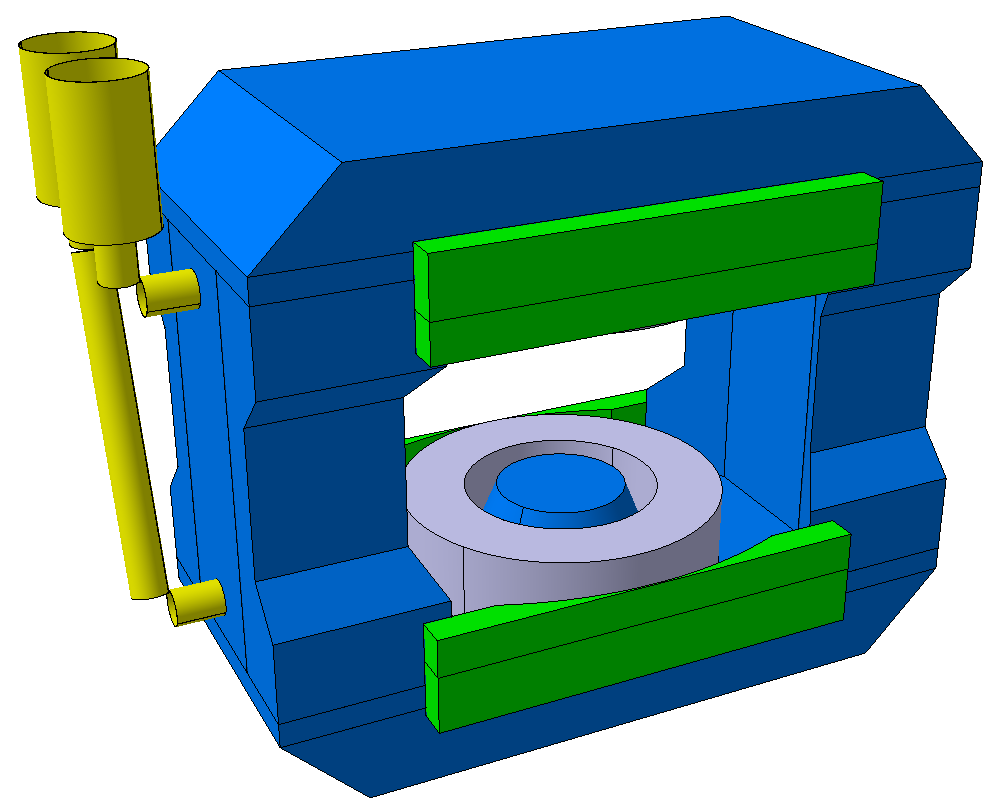
\includegraphics[width=0.7\textwidth]{pictures/New_CBM_magnet.png}
\caption{}
\label{fig:NewCbmMagnet1}
\end{figure}

\subsection{GLAD}

\begin{figure}[H]
\begin{minipage}[b]{0.495\textwidth}
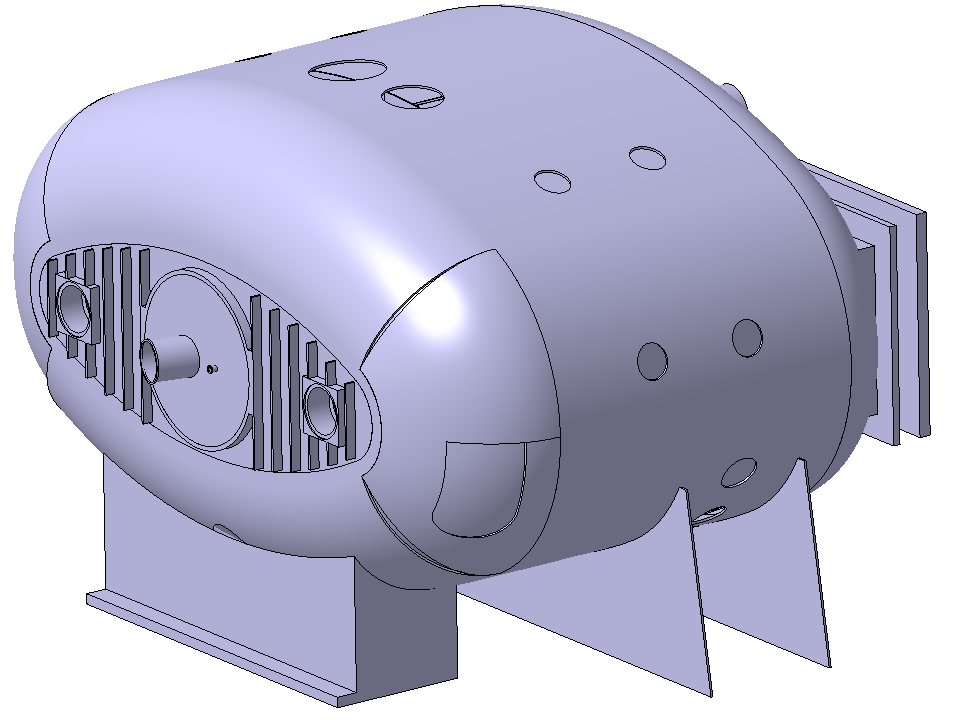
\includegraphics[width=0.95\textwidth]{pictures/GLAD1.png}
\caption{}
\label{fig:GLAD1}
\end{minipage}
\hspace{0.01\textwidth}
\begin{minipage}[b]{0.495\textwidth}
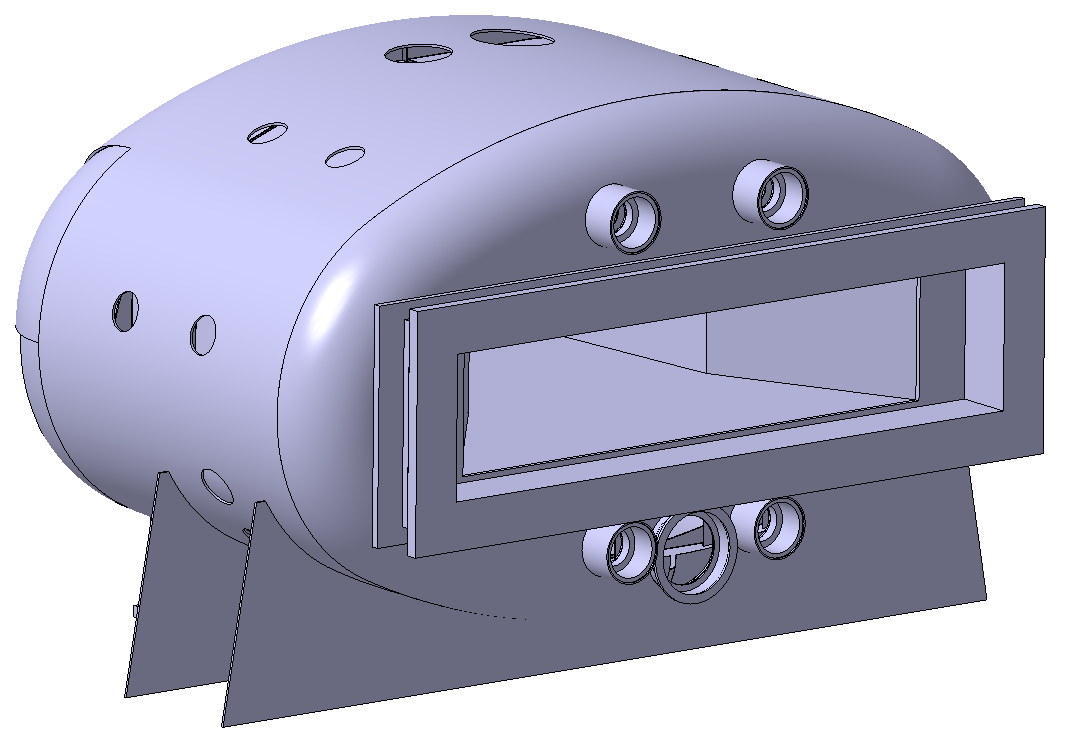
\includegraphics[width=0.95\textwidth]{pictures/GLAD2.png}
\caption{}
\label{fig:GLAD2}
\end{minipage}

\begin{minipage}[b]{0.495\textwidth}
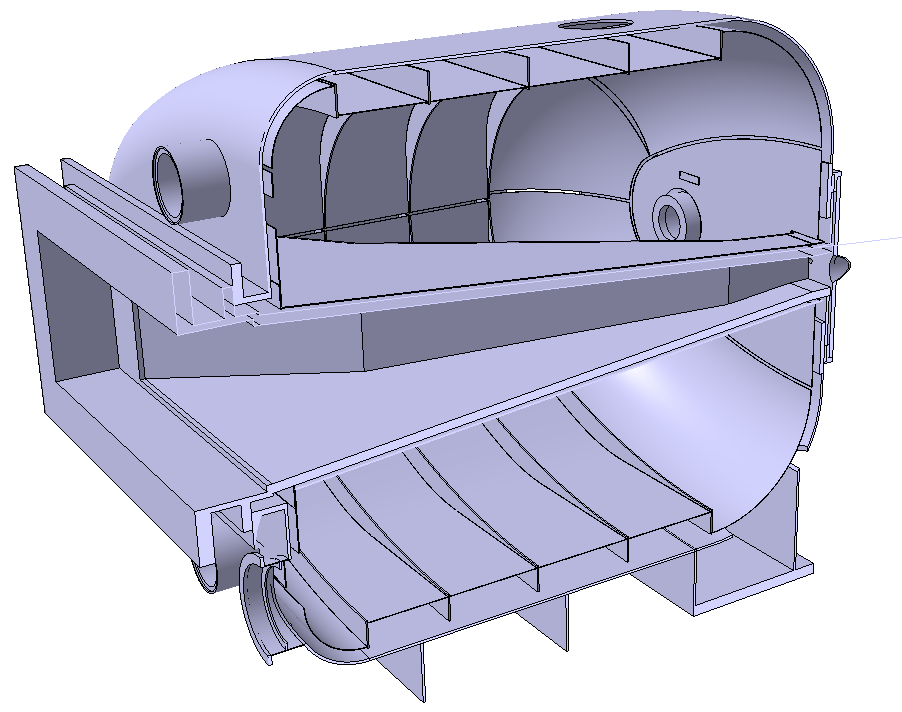
\includegraphics[width=0.95\textwidth]{pictures/GLAD3.png}
\caption{}
\label{fig:GLAD3}
\end{minipage}
\hspace{0.01\textwidth}
\begin{minipage}[b]{0.495\textwidth}
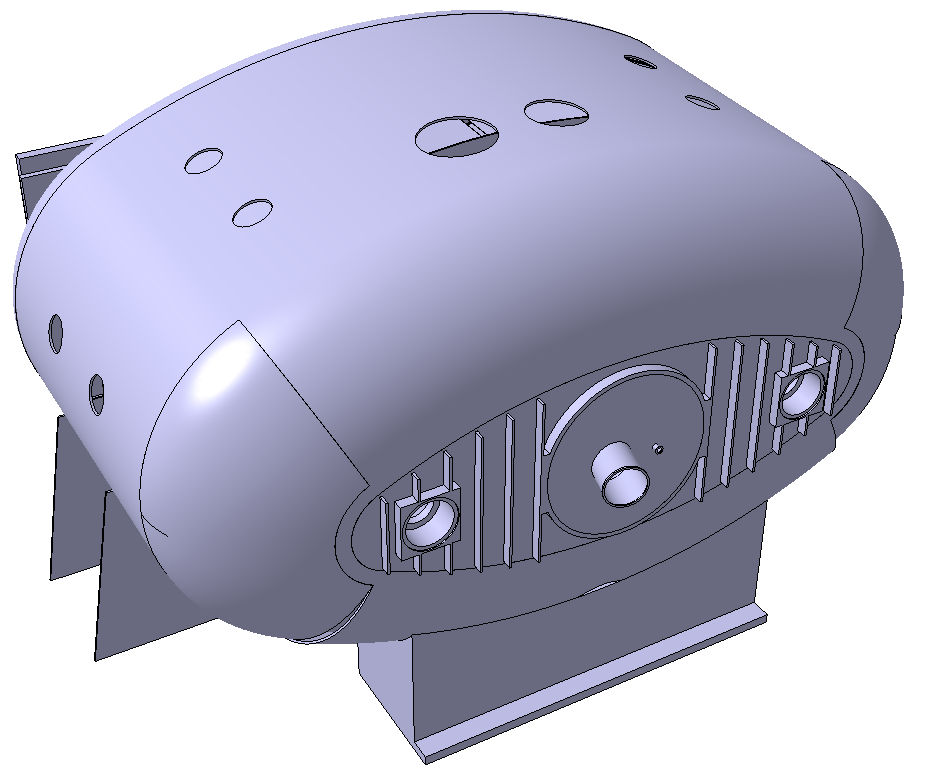
\includegraphics[width=0.95\textwidth]{pictures/GLAD4.png}
\caption{}
\label{fig:GLAD4}
\end{minipage}
\end{figure}

\subsection{CMS MUON}

\begin{figure}[H]
\centering
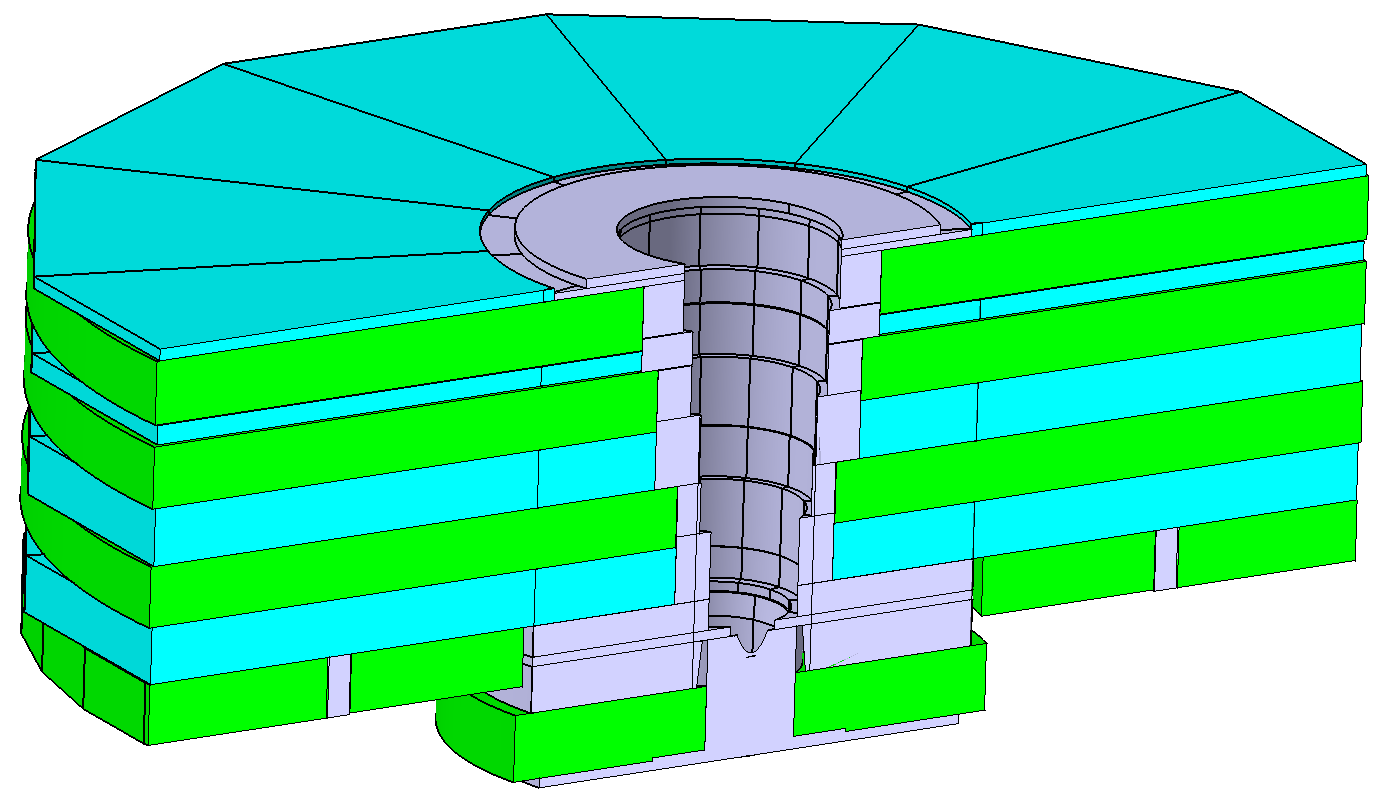
\includegraphics[width=0.7\textwidth]{pictures/CMS_MUON.png}
\caption{}
\label{fig:CmsMuon}
\end{figure}

\subsection{PANDA MUON}

Цилиндрическая часть мюонной системы эксперимента PANDA.

\begin{figure}[H]
\centering
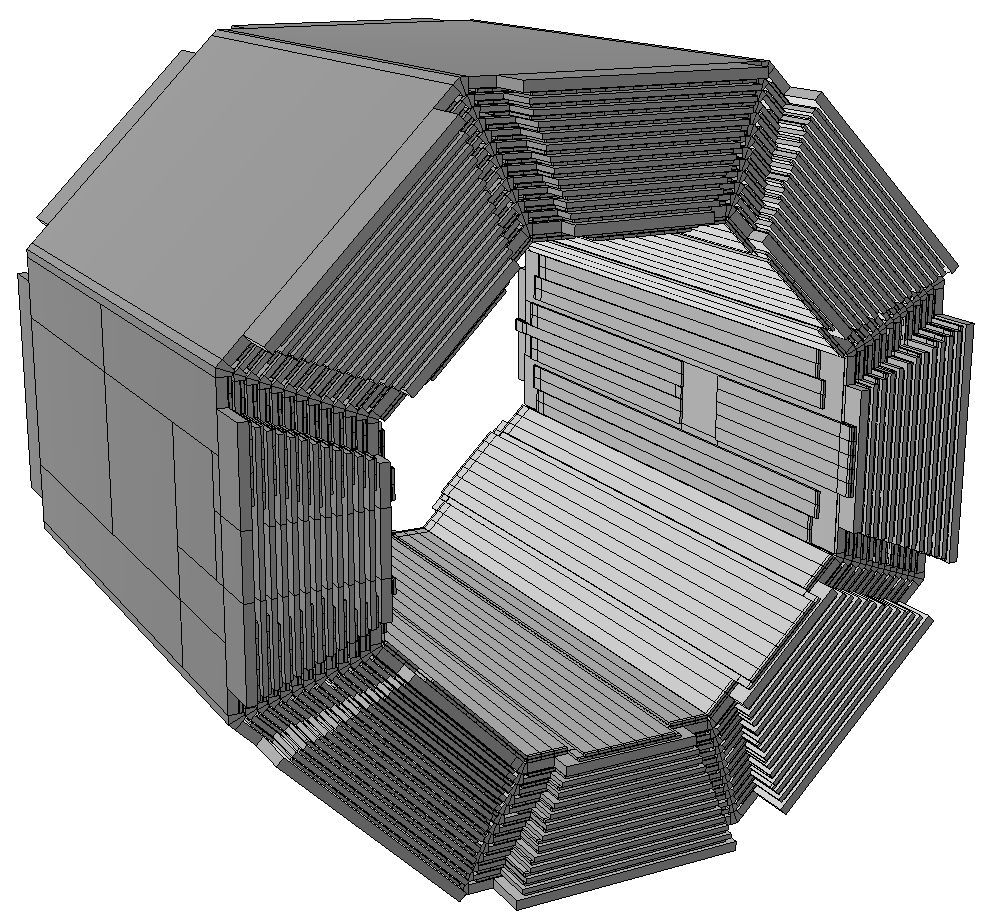
\includegraphics[width=0.7\textwidth]{pictures/PANDA_MUON_barrel.png}
\caption{}
\label{fig:PandaMuonBarrel}
\end{figure}

